\documentclass{beamer}

\usetheme{Madrid}
\usecolortheme{default}

\usepackage[utf8]{inputenc}
\usepackage[T1]{fontenc}
\usepackage[portuguese]{babel}
\usepackage{hyperref}
\usepackage{graphicx}
\usepackage{booktabs}
\hypersetup{colorlinks=true, urlcolor=blue}

\title[Momento 4: Modelação e Resultados]{Preços de Combustíveis em Portugal: Modelação e Interpretação de Resultados}
\subtitle{Momento 4 -- Modelação, Resultados e Conclusões}
\author{Tomás Oliveira}
\institute[UFP]{Seminário de Sistemas e Aplicações \\ Mestrado em Engenharia Informática -- UFP}
\date{2026/2027}

\begin{document}

% ---------- Slide 1: Título ----------
\begin{frame}
  \titlepage
\end{frame}

% ---------- Slide 2: Sumário ----------
\begin{frame}{Sumário}
  \tableofcontents
\end{frame}

% ---------- Slide 3: Recapitulação / pergunta de investigação ----------
\section{Recapitulação}
\begin{frame}{Da Exploração à Modelação}
  \textbf{O que vimos no Momento 3:}
  \begin{itemize}
    \item Forte correlação entre o Brent e o preço nacional (0,65 a 0,92 consoante o combustível).
    \item O ISP representa entre 30\% e 40\% do preço final.
    \item Padrões distintos entre variantes \emph{simples} e \emph{especial}.
  \end{itemize}
  \vspace{0.4cm}
  \textbf{Pergunta de investigação (Momento 4):}
  \begin{quote}
    É possível estimar o preço de venda ao público a partir do preço do petróleo Brent e do imposto (ISP), e qual o peso relativo de cada fator?
  \end{quote}
\end{frame}

% ---------- Slide 4: Especificação do modelo ----------
\section{Especificação do Modelo}
\begin{frame}{Modelo de Regressão Linear Múltipla}
  Foi ajustado um modelo por tipo/variante de combustível (4 modelos no total):
  \vspace{0.2cm}
  \begin{center}
    \texttt{preco\_eur\_l \textasciitilde\ brent\_eur\_litro + isp\_total\_eur\_l}
  \end{center}
  \vspace{0.3cm}
  \begin{itemize}
    \item \textbf{Variável dependente:} preço final ao público (€/litro).
    \item \textbf{Variáveis explicativas:} Brent convertido para €/litro; valor do ISP (€/litro).
    \item \textbf{Método:} mínimos quadrados ordinários (\texttt{lm()} em R).
    \item \textbf{Pacote de apoio:} \texttt{broom} -- extração de coeficientes (\texttt{tidy}), qualidade do ajuste (\texttt{glance}) e resíduos (\texttt{augment}).
    \item Um modelo \textbf{separado} por combustível/variante, para captar dinâmicas próprias de cada mercado.
  \end{itemize}
\end{frame}

% ---------- Slide 5: Tabela de resultados ----------
\section{Resultados}
\begin{frame}{Resultados dos Modelos}
  \small
  \begin{table}
    \centering
    \begin{tabular}{lrrr}
      \toprule
      Combustível & R\textsuperscript{2} & Coef. Brent & Coef. ISP \\
      \midrule
      Gasóleo especial & 0,620 & 1,487 & 1,898 \\
      Gasóleo simples & 0,816 & 2,000 & 0,449 \\
      Gasolina 95 especial & 0,542 & 1,047 & 0,429 \\
      Gasolina 95 simples & 0,852 & 1,488 & -0,090 \\
      \bottomrule
    \end{tabular}
  \end{table}
  \vspace{0.3cm}
  \footnotesize{Todos os coeficientes de Brent são estatisticamente muito significativos (p < 0,001). Fonte: \texttt{m4\_tabela\_resumo.csv}.}
\end{frame}

% ---------- Slide 6: Interpretação do R2 ----------
\begin{frame}{Interpretação: Qualidade do Ajuste (R\textsuperscript{2})}
  \begin{itemize}
    \item As variantes \textbf{simples} apresentam R\textsuperscript{2} mais elevado (0,82 -- 0,85): o preço segue de perto a lógica custo (Brent) + imposto (ISP).
    \item As variantes \textbf{especial} (premium) têm R\textsuperscript{2} mais baixo (0,54 -- 0,62): há mais variação explicada por outros fatores não incluídos no modelo -- margens de marca, posicionamento, custos de distribuição/marketing.
    \item Em todos os casos, o modelo é estatisticamente significativo (p-value praticamente nulo), confirmando que Brent e ISP são preditores relevantes.
  \end{itemize}
\end{frame}

% ---------- Slide 7: Interpretação dos coeficientes ----------
\begin{frame}{Interpretação dos Coeficientes}
  \begin{itemize}
    \item \textbf{Coeficiente do Brent} (1,0 a 2,0): por cada €1/litro de subida no Brent, o preço final sobe entre ~1,0 e ~2,0€ -- confirma repasse (e em alguns casos amplificação) do custo da matéria-prima ao consumidor.
    \item \textbf{Coeficiente do ISP} (gasóleo): positivo e elevado (0,45 a 1,90) -- o imposto tem repercussão direta e relevante no preço, especialmente no gasóleo especial.
    \item \textbf{Caso atípico -- gasolina 95 simples:} coeficiente do ISP ligeiramente negativo (-0,09), estatisticamente pouco relevante face ao peso dominante do Brent (R\textsuperscript{2}=0,85). Possível explicação: colinearidade entre Brent e ISP ao longo do tempo, e o ISP variar pouco/em degraus -- tornando o seu coeficiente instável neste modelo.
  \end{itemize}
\end{frame}

% ---------- Slide 8: Diagnóstico - resíduos ----------
\section{Diagnóstico do Modelo}
\begin{frame}{Diagnóstico: Resíduos}
  \begin{columns}
    \column{0.5\textwidth}
      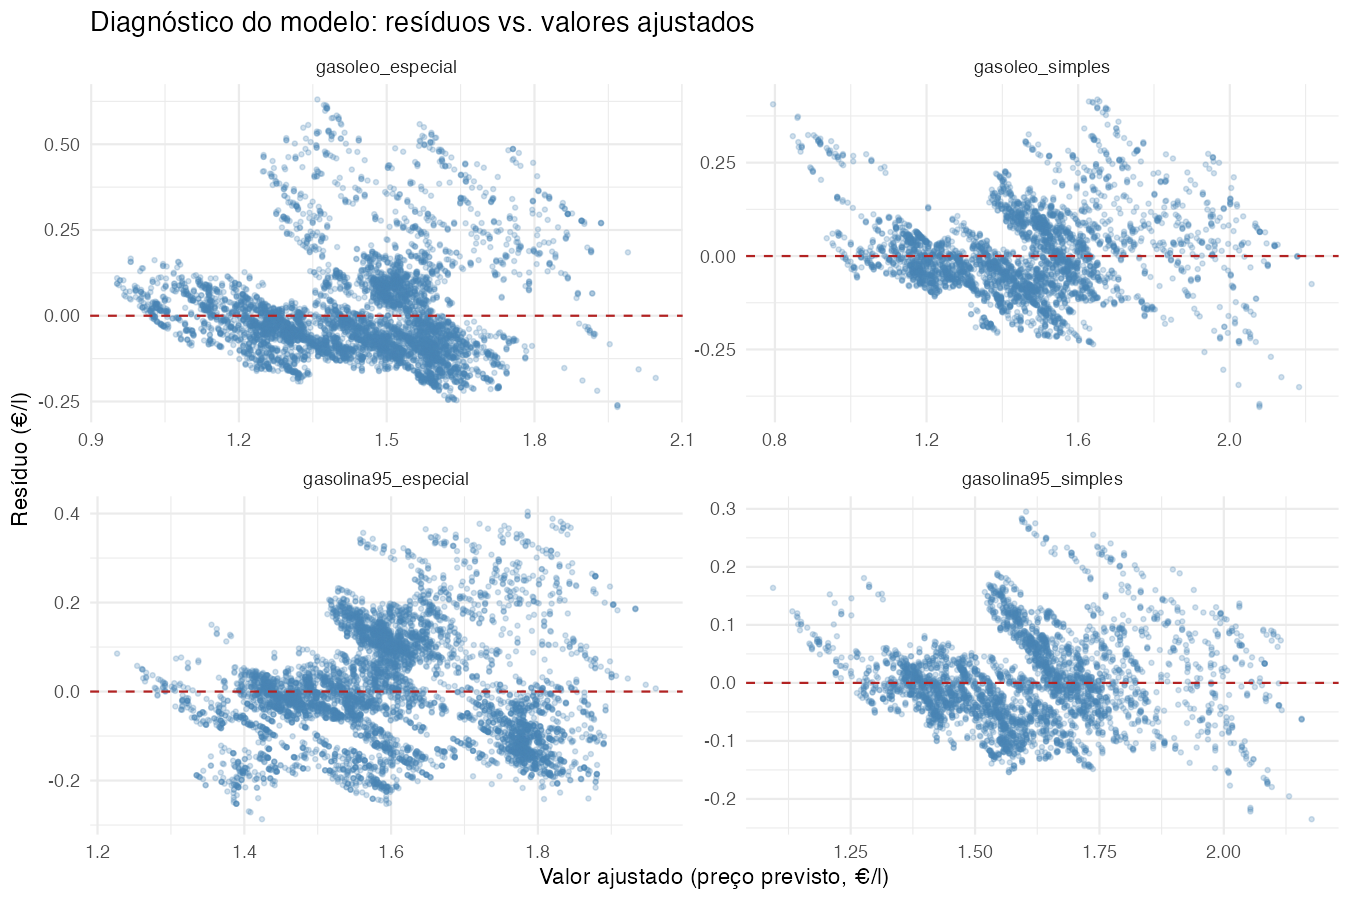
\includegraphics[width=\textwidth]{figures/m4_01_residuos_vs_ajustados.png}
    \column{0.5\textwidth}
      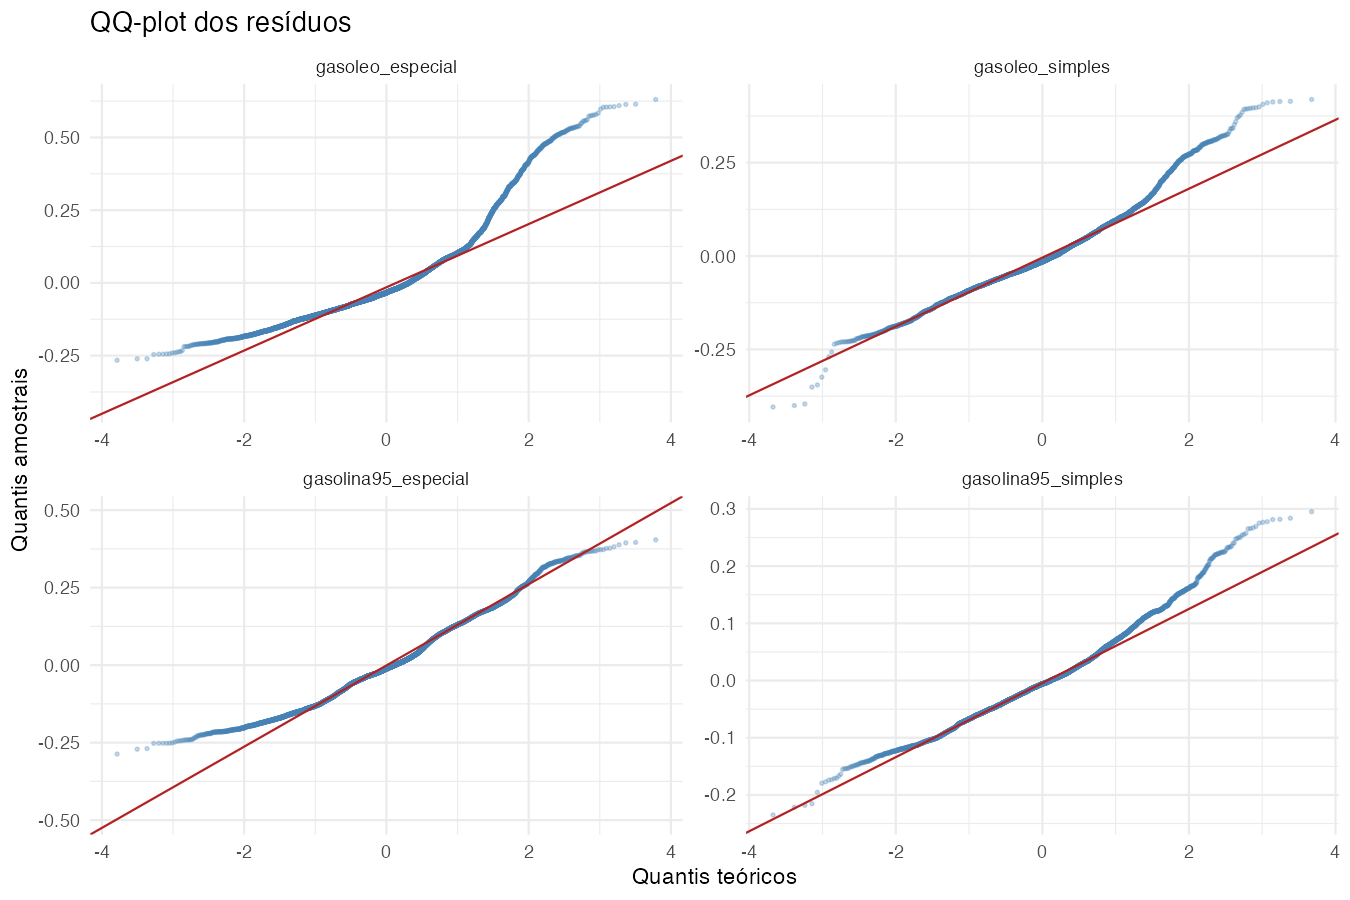
\includegraphics[width=\textwidth]{figures/m4_02_qqplot_residuos.png}
  \end{columns}
  \vspace{0.2cm}
  \footnotesize{Esquerda: resíduos vs. valores ajustados (homocedasticidade). Direita: QQ-plot dos resíduos (normalidade). Ligeiros desvios nas caudas são expectáveis dada a presença de choques pontuais (crises energéticas).}
\end{frame}

% ---------- Slide 9: Real vs Previsto ----------
\begin{frame}{Valores Reais vs. Previstos}
  \begin{center}
    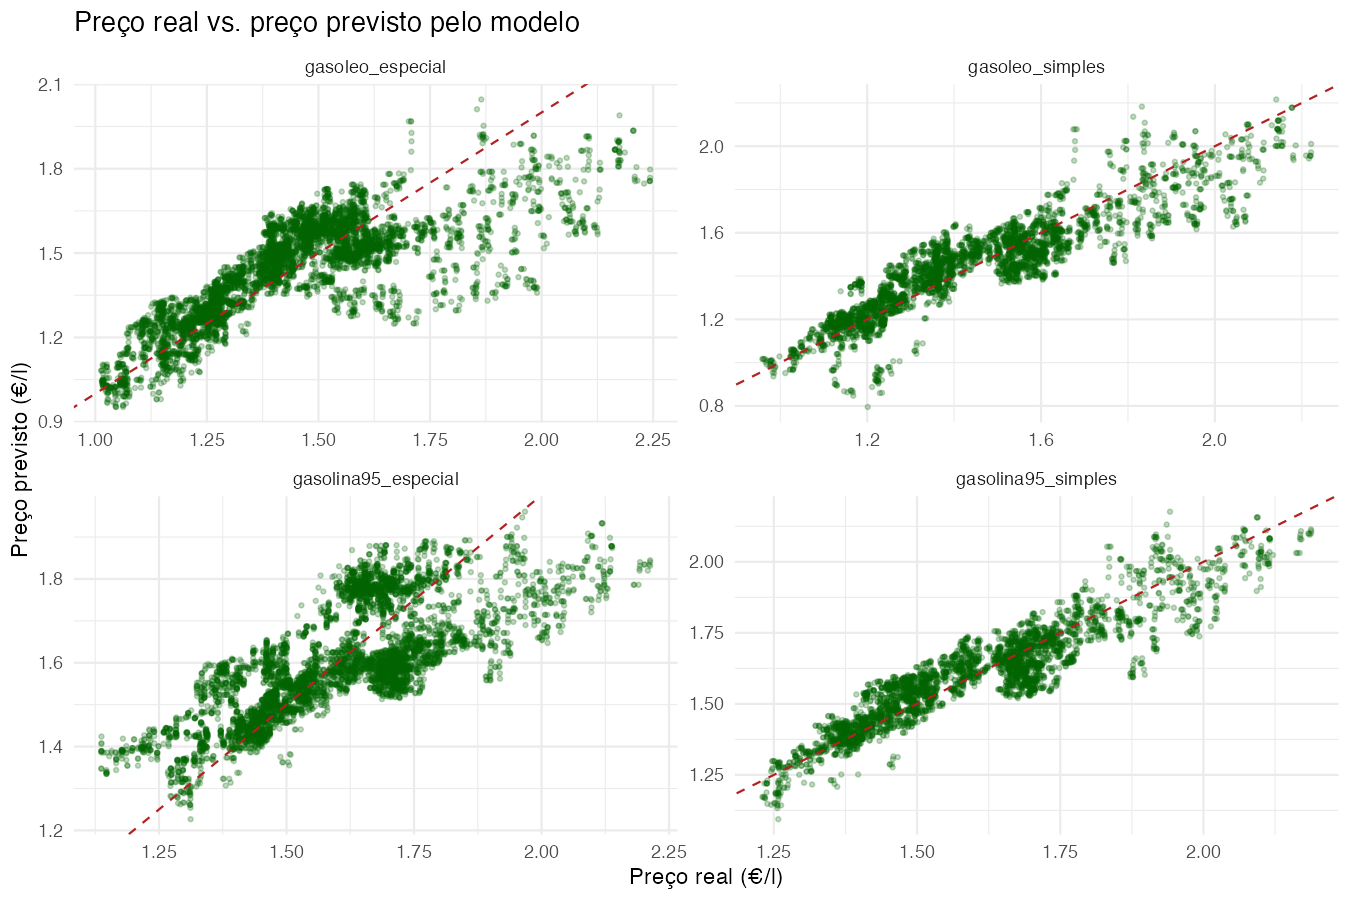
\includegraphics[width=0.75\textwidth]{figures/m4_03_real_vs_previsto.png}
  \end{center}
  \footnotesize{Os pontos próximos da reta y=x indicam bom ajuste geral do modelo, com maior dispersão nas variantes especiais.}
\end{frame}

% ---------- Slide 10: Limitações ----------
\section{Limitações}
\begin{frame}{Limitações do Modelo}
  \begin{itemize}
    \item \textbf{Multicolinearidade:} Brent e ISP não são totalmente independentes ao longo do tempo (ex.: alterações fiscais coincidentes com períodos de preços altos).
    \item \textbf{Linearidade assumida:} a relação real pode não ser perfeitamente linear (ex.: margens que se ajustam de forma não-proporcional).
    \item \textbf{Variáveis omitidas:} custos de distribuição, concorrência local, câmbio EUR/USD, e decisões de pricing das marcas não estão no modelo.
    \item \textbf{Dados limitados} para variantes \emph{simples} (apenas a partir de 2015).
    \item Não foi feita validação treino/teste formal (recomendado como trabalho futuro).
  \end{itemize}
\end{frame}

% ---------- Slide 11: Conclusões ----------
\section{Conclusões}
\begin{frame}{Conclusões}
  \begin{itemize}
    \item O Brent e o ISP explicam, em conjunto, uma parte substancial da variação dos preços dos combustíveis em Portugal (R\textsuperscript{2} entre 0,54 e 0,85).
    \item O efeito do Brent é consistentemente forte e significativo em todos os combustíveis.
    \item O peso do ISP é mais relevante no gasóleo do que na gasolina, e mais relevante nas variantes especiais.
    \item As variantes \emph{simples} seguem mais fielmente a lógica custo+imposto; as \emph{especial} têm maior margem de fatores não observados.
    \item Resultados coerentes com a literatura: preços de combustíveis dependem fortemente do petróleo bruto, mas a estrutura fiscal e as práticas comerciais introduzem variação adicional.
  \end{itemize}
\end{frame}

% ---------- Slide 12: Obrigado ----------
\begin{frame}
  \centering
  \Huge{Obrigado!}

  \vspace{0.5cm}
  \Large{Perguntas?}
\end{frame}

\end{document}
